\documentclass[11pt]{article}
\usepackage{fullpage}
\usepackage{listings}
\usepackage{needspace}
\usepackage{color}
\usepackage{ifthen}
\usepackage{pgf}
\usepackage{tikz}
\usetikzlibrary{arrows,automata,shapes}
\usepackage{amsmath}
\usepackage{url}
\usepackage{framed}
\usepackage{csc}
\usepackage{textcomp}

\lstset{ %
basicstyle=\footnotesize\ttfamily,       % the size of the fonts that are used for the code
numbers=left,                   % where to put the line-numbers
stepnumber=1,                   % the step between two line-numbers. If it's 1 each line will be numbered
numbersep=5pt,                  % how far the line-numbers are from the code
showspaces=false,               % show spaces adding particular underscores
showstringspaces=false,         % underline spaces within strings
tabsize=4,		                % sets default tabsize to 4 spaces
language=Python,
upquote=true,
columns=fixed
}

\ifthenelse{\isundefined{\isAnswerKey}}
{
    \newenvironment{answer}{\large\lstset{basicstyle=\large}\color{white}}{}
}
{
    \newenvironment{answer}{\large\lstset{basicstyle=\large}\color{red}}{}
}


\author{Computer Science Community}
\title{CS-141 Final Exam Review}
\date{\today}

\makeatletter
\let\thetitle\@title
\let\theauthor\@author
\let\thedate\@date
\makeatother

\begin{document}
\header

% TODO (TOFU) copy in Chris's marvelous mixture from the old 241 Final
\begin{enumerate}


    \item You are given the linked list: $1 \rightarrow 2 \rightarrow 3$.  You may assume that each node has one field called \texttt{value} and one called \texttt{next}.
        \begin{enumerate}
            \item 1 points to 2 and 2 points to 3. What does 3 point to?
                \begin{answer}
				The implementer may cause the 3 node to point to either \textit{None} or a sentinel node.
				\end{answer}
            \item Draw out the linked list structure and add a 5 to the end.
				\begin{answer}
				\leftmargin=0em
				\itemindent=0em
				{ \small
				\begin{verbatim}
+----------+    +----------+    +----------+    +------------+
| value: 1 |    | value: 2 |    | value: 3 |    | value: 5   |
| next: ------->| next: ------->| next: ------->| next: None |
+----------+    +----------+    +----------+    +------------+
				\end{verbatim}
				\textit{OR}
				\begin{verbatim}
+----------+    +----------+    +----------+    +----------+    +-----------------+
| value: 1 |    | value: 2 |    | value: 3 |    | value: 5 |    | value: SENTINEL |
| next: ------->| next: ------->| next: ------->| next: ------->|                 |
+----------+    +----------+    +----------+    +----------+    +-----------------+
				\end{verbatim} }
				\end{answer}
            \item Write pseudocode to add an element onto the end of a linked list.
				\begin{answer}
				\begin{lstlisting}
def append(value, llist):
	newend := new node
	newend.value := value
	newend.next := None
	curend := end of llist
	curend.next := newend
				\end{lstlisting}
				\end{answer}
            \pagebreak
            \item Looking at the list from (b), you notice that we forgot to
                  add in a 4. What is a procedure for doing this? (There are
                  many possibilities.) \\
                \begin{answer}
				Use some variation of this procedure: Find the preceding element's node (in this case, 3), link its next node to the new node containing 4, then link that new node to what was the following node.
				\end{answer}
        \end{enumerate}
    \item Write a Python function, given a sorted linked list, returns a Python
    list of all of the elements which are in the list more than once. (eg.
    $1\rightarrow2\rightarrow2\rightarrow3\rightarrow3\rightarrow3$ would return [2,3,3] )
        \vspace{3in}
\begin{answer}
\begin{lstlisting}
def find_dupes(node):
	dup = []
	while node.next != None:
		if node.value == node.next.value:
			val = node.value
			dup.append(val)
			while node.value == val:
				node = node.next
				if node == None:
					return dup
		node = node.next
	return dup
\end{lstlisting}
\end{answer}
    \item If your solution to (3) was iterative, write it recursively; if it
    was recursive, write it iteratively.
\begin{answer}
\begin{lstlisting}
def find_dupes(node, dup=[], ignore=False):
	if node.next == None:
		return dup
	if not ignore and node.value == node.next.value:
		dup.append(node.value)
	return find_dupes(node.next, dup, node.value == node.next.value)
\end{lstlisting}
\end{answer}
        \pagebreak

\section*{Stacks and Queues}
\item How can you use a stack to determine if an input string has properly
      balanced parens, brackets and braces. (eg. ``[\{\}]'' is accepted, but
      ``(()'' and ``[(])'' are not)?

    \begin{answer}
    \begin{lstlisting} 
def delims_are_balanced(inString):
    ''' String -> boolean
    Determines if the input string has balanced delimiters
    Delimiters are () [] {} and <>  
    
    '''
    delim = {'(': ')', '[': ']', '{': '}', '<': '>'}
    stack = Stack()
    for char in inString:
        if char in delim:
            stack.push(char)
        elif char in delim.values():
            if stack.is_empty():
                return False
            if delim[stack.peek()] == char:
                stack.pop()
            else:
                return False
    return stack.is_empty()
    \end{lstlisting}
    \end{answer}

\item If we wanted to implement a stack as a linked list, what linked-list
	operations would correspond to push() and pop()?

	\begin{answer}
	push( stack, element ) $\rightarrow$ insertFront( linked-list, element )\\
	pop( stack ) $\rightarrow$ removeFront( linked-list )
	\end{answer}
	
\item Write your own stack class using python's built in lists to manage the elements of your stack. \\
Your stack must provide the following functionality:
	  \begin{itemize}
	  \item []push( elm ) - push elm onto the top of the stack
	  \item []pop() - return the top elm of the stack and remove it from the stack
	  \item []isEmpty() - is the stack empty()
	  \item []peek() - which returns the top element of the stack without modifying the stack. 
	  \item []\_\_str\_\_
	  \end{itemize}
	  \begin{answer}
	  \begin{lstlisting}
	  class Stack:
		def __init__(self):
			self.lst = []
		def push(self, val ):
			self.lst.append( val )
		def pop(self):
			return self.lst.pop()
		def peek(self):
			return self.lst[-1]
		def isEmpty(self):
			return (len(self.lst) == 0)
		def __str__(self):
			return str(self.lst)
			  \end{lstlisting}
	  \end{answer}

\section*{Backtracking}

\item Why is backtracking better suited for solving a Sudoku puzzle than
      using regular brute force?

    \begin{answer}
    A properly implemented backtracking approach will prune fruitless branches. 
    \end{answer}

\pagebreak
\section*{Hashing and Hash Tables}

\item Chris made a mistake in his hashtable implementation!

    \lstinputlisting{code/wonkyhash.py}
    \begin{enumerate}
    \item Show what the hashtable looks like after the for loop on line 24
          completes. 

        \begin{answer}
		\begin{lstlisting}[numbers=none]
[once, a, [], []]
		\end{lstlisting}

        \end{answer}

    \item What is wrong with the code? What can we do to make the function behave as Chris expects it to behave?

        \begin{answer}
        The issue is on line 6. This line overwrites the list the element, things are getting overwritten and the contains method will break. Change 
\begin{lstlisting}[numbers=none]
self.table[self.bad_hash(element)] = element 
\end{lstlisting} to 
\begin{lstlisting}[numbers=none]
self.table[self.bad_hash(element)].append(element)
\end{lstlisting}

        \end{answer}

    \item Draw the table of the properly behaving hash function.
        
        \begin{answer}
		\begin{lstlisting}[numbers=none]
[['wrestled', 'bear', 'once'], ['I', 'a'], [], []]
		\end{lstlisting}
    \end{answer}
\item Assuming that this hashtable will only be used on strings, is the hashing function being used a good one? Why or why not?

    \begin{answer}
        No, it ignores the fact that most english words are the roughly the same length. The number of collisions is expected to be massive. We should take advantage of the characters in the input strings, not the number of characters.
    \end{answer}
    \end{enumerate}


\section*{Sorting}

\item Fill in the table for the asymptotic running time of each sorting
      algorithm.
      \begin{center}
      \begin{tabular}{|r|c|c|c|}
        \hline
        ~ & Best & Worst & Average \\\hline
        MergeSort &
            \begin{answer}$O(n*\textrm{log}(n))$\end{answer} &
            \begin{answer}$O(n*\textrm{log}(n))$\end{answer} &
            \begin{answer}$O(n*\textrm{log}(n))$\end{answer} \\\hline
        Quicksort &
            \begin{answer}$O(n*\textrm{log}(n))$\end{answer} &
            \begin{answer}$O(n^2)$\end{answer} &
            \begin{answer}$O(n*\textrm{log}(n))$\end{answer} \\\hline
        HeapSort &
            \begin{answer}$O(n*\textrm{log}(n))$\end{answer} &
            \begin{answer}$O(n*\textrm{log}(n))$\end{answer} &
            \begin{answer}$O(n*\textrm{log}(n))$\end{answer} \\\hline
      \end{tabular}
      \end{center}

\item What sorting algorithm splits its input list into two other lists, one
      which has element which are all smaller than a value (which is randomly
      selected) and one which has elements which are all larger than the
      randomly selected value?

    \begin{answer}
    Quicksort.
    \end{answer}

\item\label{qsort-worst-case} What kind of data causes Quicksort's worst-case
      time complexity? You may assume that we always pick the first element as
      the pivot.

      \begin{answer}
      Data that is (nearly) sorted or is sorted in reverse order.
      \end{answer}

\item What causes Quicksort to run so slowly on the input you describe in
      question \ref{qsort-worst-case}?

    \begin{answer}
    Quicksort splits its input into two lists based on the value of the pivot.
    If the pivot is either the smallest or the largest element, then one list
    will only have no elements, while the others will have all of the elements
    but the pivot. We can see this if we perform a substitution trace:

\begin{verbatim}
qsort([1,2,3,4])
qsort([]) + [1] + qsort([2,3,4])
qsort([]) + [1] + qsort([]) + [2] + qsort([3,4])
qsort([]) + [1] + qsort([]) + [2] + qsort([]) + [3] + qsort([4])
qsort([]) + [1] + qsort([]) + [2] + qsort([]) + [3] + qsort([4])
qsort([]) + [1] + qsort([]) + [2] + qsort([]) + [3] + qsort([]) + [4] + qsort([])
[1,2,3,4]
\end{verbatim}
    \end{answer}

\item In Quicksort, why do we select a random pivot value, rather than always
      pivoting on the first element?

      \begin{answer}
      With real-world data, we're more likely to encounter ordered or
      semi-ordered data than randomised data. This makes it more likely for us
      run into Quicksort's worst-case time complexity. We run into this bad
      time complexity if we select pivots which are near the lowest or highest
      values.

      Selecting a random value to pivot on helps us encounter the average case
      evens out the distribution of ordered and unordered data. Even if we're
      getting in sorted data, if we select pivots randomly, we should be able
      to end up with average time complexity.
      \end{answer}

\pagebreak
\item Show the stages of a Merge sort and a Quicksort on the following list:
      [3,5,1,3,2,7,9]. Be sure to identify your pivot.

    \begin{answer}
	Mergesort:\\*
	\newline
    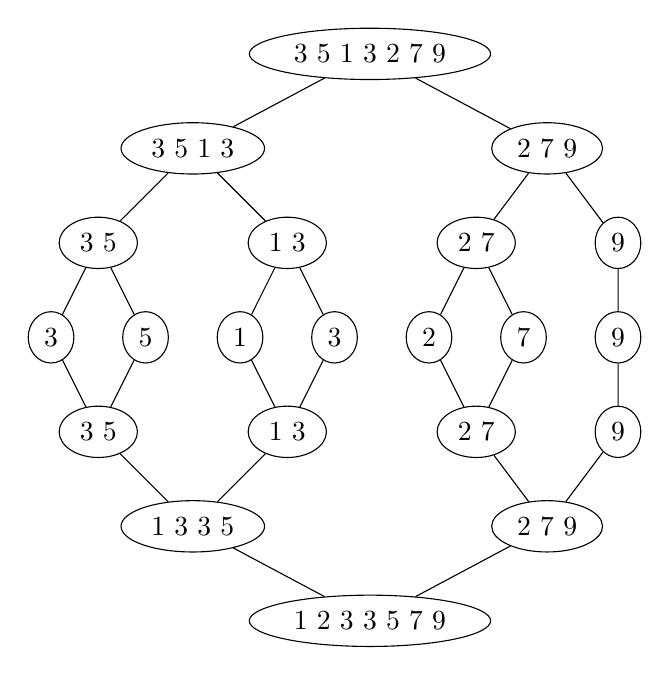
\begin{tikzpicture}[scale=1.2]
	\node [draw,ellipse] at (3.375,3) (head) {3 5 1 3 2 7 9};
	\node [draw,ellipse] at (1.5,2) (1) {3 5 1 3};
	\node [draw,ellipse] at (5.25,2) (2) {2 7 9};
	\node [draw,ellipse] at (.5,1) (3) {3 5};
	\node [draw,ellipse] at (2.5,1) (4) {1 3};
	\node [draw,ellipse] at (4.5,1) (5) {2 7};
	\node [draw,ellipse] at (6,1) (6) {9};
	\node [draw,ellipse] at (0,0) (7) {3};
	\node [draw,ellipse] at (1,0) (8) {5};
	\node [draw,ellipse] at (2,0) (9) {1};
	\node [draw,ellipse] at (3,0) (10) {3};
	\node [draw,ellipse] at (4,0) (11) {2};
	\node [draw,ellipse] at (5,0) (12) {7};
	\node [draw,ellipse] at (6,0) (13) {9};
	\node [draw,ellipse] at (.5,-1) (14) {3 5};
	\node [draw,ellipse] at (2.5,-1) (15) {1 3};
	\node [draw,ellipse] at (4.5,-1) (16) {2 7};
	\node [draw,ellipse] at (6,-1) (17) {9};
	\node [draw,ellipse] at (1.5, -2) (18) {1 3 3 5};
	\node [draw,ellipse] at (5.25, -2) (19) {2 7 9};
	\node [draw,ellipse] at (3.375,-3) (20) {1 2 3 3 5 7 9};

	\path [draw] (1) -- (head) -- (2);
	\path [draw] (3) -- (1) -- (4);
	\path [draw] (5) -- (2) -- (6);
	\path [draw] (7) -- (3) -- (8);
	\path [draw] (9) -- (4) -- (10);
	\path [draw] (11) -- (5) -- (12);
	\path [draw] (13) -- (6);
	\path [draw] (7) -- (14) -- (8);
	\path [draw] (9) -- (15) -- (10);
	\path [draw] (11) -- (16) -- (12);
	\path [draw] (13) -- (17);
	\path [draw] (14) -- (18) -- (15);
	\path [draw] (16) -- (19) -- (17);
	\path [draw] (18) -- (20) -- (19);
	\end{tikzpicture}\\*
	\newline
	Quicksort (using the first element in the list as a pivot):\\*
	\newline
	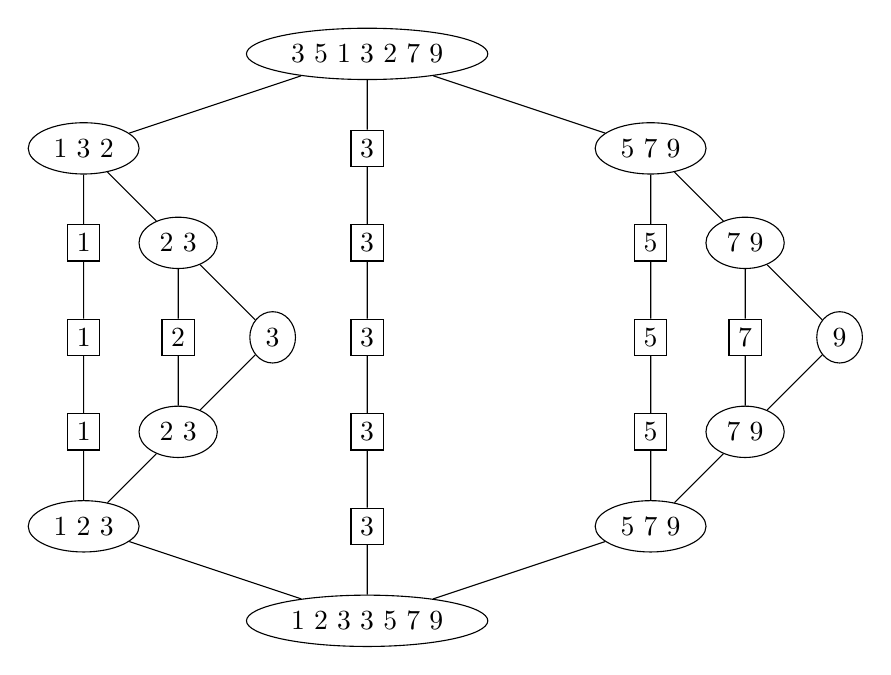
\begin{tikzpicture}[scale=1.2]
	\node [draw] at (1,0) (1) {1};
	\node [draw] at (2,0) (2) {2};
	\node [draw,ellipse] at (3,0) (3) {3};
	\node [draw] at (4,0) (4) {3};
	\node [draw] at (7,0) (5) {5};
	\node [draw] at (8,0) (6) {7};
	\node [draw,ellipse] at (9,0) (7) {9};
	\node [draw] at (1,1) (8) {1};
	\node [draw, ellipse] at (2,1) (9) {2 3};
	\node [draw] at (4,1) (10) {3};
	\node [draw] at (7,1) (11) {5};
	\node [draw,ellipse] at (8,1) (12) {7 9};
	\node [draw, ellipse] at (1,2) (13) {1 3 2};
	\node [draw] at (4,2) (14) {3};
	\node [draw,ellipse] at (7,2) (15) {5 7 9};
	\node [draw,ellipse] at (4,3) (16) {3 5 1 3 2 7 9};
	\node [draw] at (1,-1) (17) {1};
	\node [draw,ellipse] at (2,-1) (18) {2 3};
	\node [draw] at (4, -1) (19) {3};
	\node [draw] at (7,-1) (20) {5};
	\node [draw, ellipse] at (8,-1) (21) {7 9};
	\node [draw, ellipse] at (1,-2) (22) {1 2 3};
	\node [draw] at (4,-2) (23) {3};
	\node [draw, ellipse] at (7,-2) (24) {5 7 9};
	\node [draw, ellipse] at (4,-3) (25) {1 2 3 3 5 7 9};

	\path [draw] (1) -- (8) -- (13);
	\path [draw] (2) -- (9);
	\path [draw] (3) -- (9) -- (13);
	\path [draw] (4) -- (10) -- (14) -- (16);
	\path [draw] (5) -- (11) -- (15);
	\path [draw] (6) -- (12);
	\path [draw] (7) -- (12) -- (15) -- (16);
	\path [draw] (13) -- (16);

	\path [draw] (1) -- (17) -- (22);
	\path [draw] (2) -- (18);
	\path [draw] (3) -- (18) -- (22) -- (25);
	\path [draw] (4) -- (19) -- (23) -- (25);
	\path [draw] (5) -- (20) -- (24);
	\path [draw] (6) -- (21);
	\path [draw] (7) -- (21) -- (24) -- (25);

	\end{tikzpicture}
    \end{answer}

\section*{Heaps and Heapsort}

\item For a binary heap containing $n$ elements, what is the maximum number of
      swaps occurring after an insert operation?

    \begin{answer}
        log$_{\textrm{2}}$ (n + 1), rounded down.
    \end{answer}

\item Given a node in an array-based binary heap at index $i$, where are the
      indices of both its children? What is the index of its parent?

    \begin{answer}
    The children are at $2i+1$ and $2i+2$. The parent is at
    $\lfloor\frac{i-1}{2}\rfloor$.

    \marginpar{\small\em Note that in a 1 indexed array system, the children
    would be at $2i$ and $2i+1$. The parent would be at
    $\lfloor\frac{i}{2}\rfloor$.}
    \end{answer}

\item Run a heap sort on the following list: [3,5,1,3,2,7,9], showing the heap
      at each stage. Be sure to heapify the list first.

    \begin{answer}
        Heapify:  \newline
        	[\underline{3}, 5, 1, 3, 2, 7, 9] \newline
    		[\underline{3},\underline{5}, 1, 3, 2, 7, 9] \newline
    		[\underline{1}, \underline{5}, \underline{3}, 3, 2, 7, 9] \newline
    		[\underline{1}, \underline{3}, \underline{3}, \underline{5}, 2, 7, 9] \newline
    		[\underline{1}, \underline{2}, \underline{3}, \underline{5}, \underline{3}, 7, 9] \newline
    		[\underline{1}, \underline{2}, \underline{3}, \underline{5}, \underline{3}, \underline{7}, 9] \newline
    		[\underline{1}, \underline{2}, \underline{3}, \underline{5}, \underline{3}, \underline{7}, \underline{9}] \newline 
    	
    	Sort: \newline
    		[\underline{2}, \underline{3}, \underline{3}, \underline{5}, \underline{9}, \underline{7}, 1] \newline
    		[\underline{3}, \underline{3}, \underline{7}, \underline{5}, \underline{9}, 2, 1] \newline
    		[\underline{3}, \underline{5}, \underline{7}, \underline{9}, 3, 2, 1] \newline
    		[\underline{5}, \underline{9}, \underline{7}, 3, 3, 2, 1] \newline
    		[\underline{7}, \underline{9}, 5, 3, 3, 2, 1] \newline
    		[\underline{9}, 7, 5, 3, 3, 2, 1] \newline
    		[9, 7, 5, 3, 3, 2, 1] \newline
    \end{answer}

\item If we have a balanced binary search tree (its height is as small as
    possible) containing 'n' nodes.
        \begin{enumerate}
            \item What is its height? \\
                \begin{answer}
                log$_2$(n)
                \end{answer}
            \item How much time would it take to traverse to any of the leaf
            nodes of this tree. \\
                \begin{answer}
                log$_2$(n)
                \end{answer}
            \item What's the worst case search time for an (unbalanced) search
            tree? \\
                \begin{answer}
                n
                \end{answer}
                \pagebreak
        \end{enumerate}
    \item Write a function that determines if a given element is in a binary search tree.
        \vspace{3in}
    \item Write a function which counts the number of leaf nodes in a given binary tree.
        \pagebreak
    \item Create a binary search tree, drawing the whole tree
        again for each element inserted from the list: [1,2,8,3,5].
        \vspace{6in}

\end{enumerate}

\end{document}
